\section{UPPAAL SMC}\label{sec:smc}
UPPAAL \gls{smc} is one of the newer versions of UPPAAL, it works with statistical model checking for more efficient analysis, as it avoids the exhaustive exploration of the state-space. This statistical exploration gives the added benefit of significantly less memory consumption\cite{cs_smc}, meaning that the computers physical memory is rarely the limit when running a query. This flexibility allows for \gls{smc} to be used for other subjects than verification such as planing\cite{cs_smc}. \\
In addition \gls{smc} have been updated so that it can handle non linear cost and differential equations which makes it possible to implement \gls{kibam}.

After having run a simulation query, it is possible to get a graph illustrating the result of running the simulations. In \cref{fig:simab} we see two variable which have been simulated five times for $15.000$ units of time, this will be useful for monitoring the battery energy levels over time.

\begin{figure}[!h]
	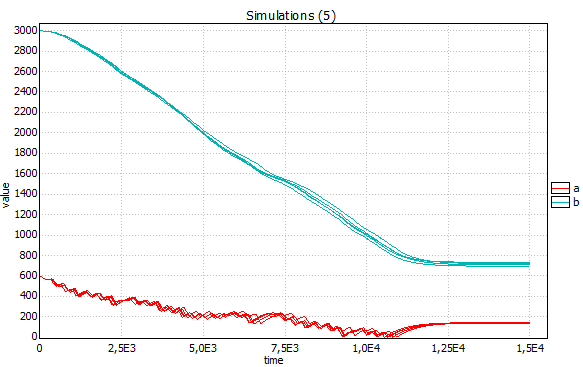
\includegraphics[width=\textwidth]{graphics/simab.png}
	\label{fig:simab}
	\caption{Five simulations of the value of two variables \uppVar{a, b} over time}
\end{figure}

Also it is possible to run probabilities queries, these answers the question; \textit{"What is the probability that some condition will be fulfilled?"}. An example of this can be seen in \cref{fig:pra300}, where we have run the probability that our variable \uppVar{a} will fall below $300$ within time $7200$. \Gls{smc} have then run this by randomly simulating the models behaviour until it with some certainty, within a specified margin of error, knows the chance of the property being true.\\
\Cref{fig:pra300} shows that prior to time $4120$ there are no chance of \uppVar{a} being under $300$, and at time $4520$ it will with certainty be under $300$. For this query it was specified that a $5\%$ uncertainty was acceptable, this resulted in the result seen in \cref{fig:pra300pct} which shows that \gls{smc} was $~90\% - 100\%$ certain \uppVar{a} would fall below $300$. The certainty parameter can be modified to become more precise, at the cost of run time as it will have to run more simulations in order to ensure the correct probability. Using the probability query also allow  for several other types graphs such as probability distribution and frequency histogram.

\begin{figure}[h]
	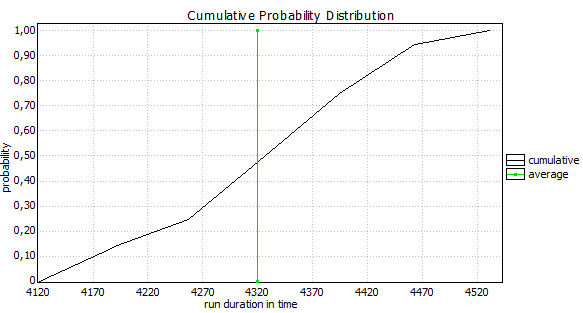
\includegraphics[width=\textwidth]{graphics/pra300.png}
	\label{fig:pra300}
	\caption{Probability over time that the value of (a) will fall under 300}
\end{figure}

\begin{figure}[h]
	\centering
	
\includegraphics[width=8cm]{graphics/pra300pct.png}
	\label{fig:pra300pct}
	\caption{Initial result of running a probability query}
\end{figure}


